% Appendix D: α sensitivity

Figure~\ref{fig:alpha_sweep} and Tab.~\ref{tab:alpha_sweep} report HCCP's empirical coverage and $\shat$-bin gap as the miscoverage level $\alpha$ sweeps over $\{0.01, 0.05, 0.10, 0.15, 0.20, 0.30, 0.50\}$, fixed feature set CADD+GPN-MSA+Borzoi, fixed $K = 5$, single seed. The target $1 - \alpha$ line is included for reference.

\begin{figure}[h]
\centering
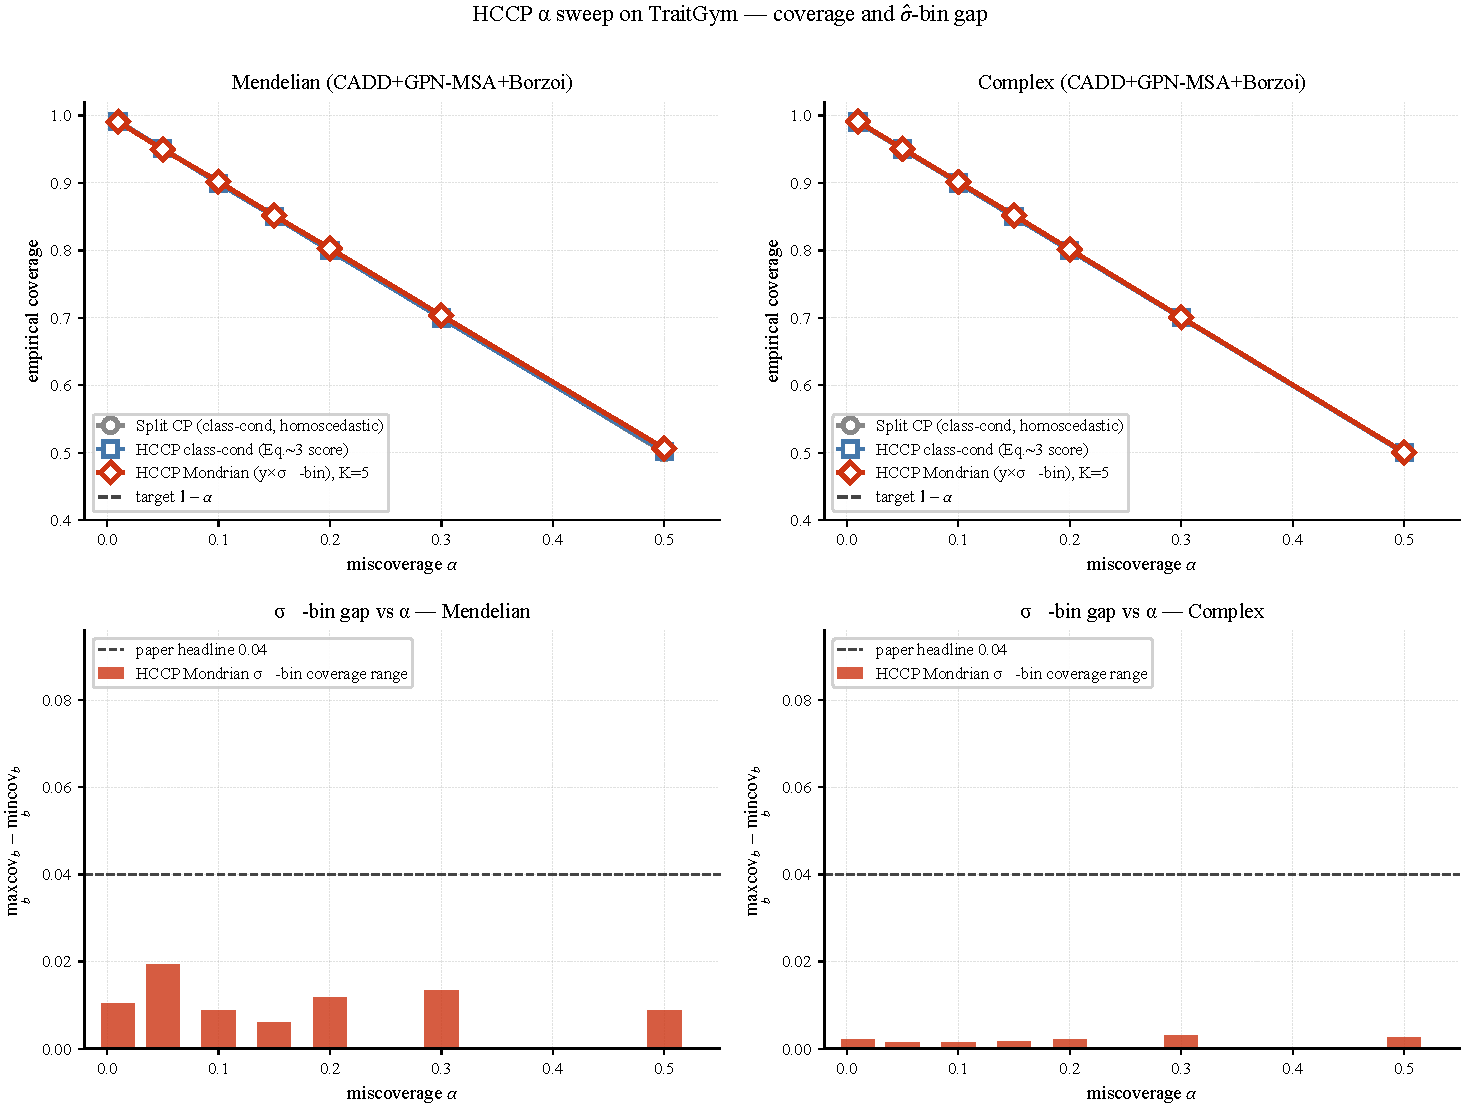
\includegraphics[width=0.95\linewidth]{figures/figD_alpha_sweep.pdf}
\caption{Compact 1$\times$3 $\alpha$-sweep with datasets encoded by line style: \emph{Mendelian} = solid line, filled markers; \emph{Complex} = dashed line, hollow markers. \textbf{(a)} Calibration residual $\mathrm{cov} - (1{-}\alpha)$ for Split CP (homoscedastic class-cond, gray), HCCP class-cond (blue), and HCCP Mondrian $(y \times \shat\text{-bin}, K{=}5)$ (red); shaded band is the finite-sample slack $\pm 1/(n_{\min}{+}1)$. All six (method $\times$ dataset) curves track target to within the slack at every $\alpha$. \textbf{(b)} $\shat$-bin coverage range $\max_b \mathrm{cov}_b - \min_b \mathrm{cov}_b$ for HCCP Mondrian, grouped per $\alpha$ (Mendelian red bars left, Complex blue bars right; numeric annotations on small Complex bars); dashed reference is the $\alpha{=}0.10$ headline threshold $\leq 0.04$, respected at every $\alpha$ on both datasets. \textbf{(c)} Singleton fraction (the operational knob); the three benchmarked operating points $\alpha \in \{0.10, 0.20, 0.30\}$ are marked by vertical guides and labeled at top — \emph{high-stakes} / \emph{triage} / \emph{hypothesis} (full operating-point recommendations in the body text below). The arrow callout marks the Mendelian non-monotonicity peak ($\approx 0.82$ at $\alpha = 0.15$): at large $\alpha$ on the imbalanced minority-class regime, empty-set abstentions $\emptyset$ replace singletons, an honest finite-sample artefact.}
\label{fig:alpha_sweep}
\end{figure}

\begin{table}[h]
\centering
\small
\caption{$\alpha$ sweep: marginal coverage, $\shat$-bin gap, and singleton fraction (Mendelian / Complex, CADD+GPN-MSA+Borzoi, $K = 5$, seed 42). HCCP maintains coverage within one finite-sample slack $1/(n_{\min}+1)$ of target across all $\alpha$. Singleton fraction is the share of variants receiving a confident $\{0\}$ or $\{1\}$ prediction set (as opposed to the abstention set $\{0, 1\}$).}
\label{tab:alpha_sweep}
% Auto-generated by scripts/28_alpha_sweep_figure.py
\begin{tabular}{rrrrrr}
\toprule
$\alpha$ & M cov & M $\hat\sigma$-gap & C cov & C $\hat\sigma$-gap & singleton (M / C)\\
\midrule
0.01 & 0.991 & 0.010 & 0.991 & 0.002 & 53\% / 3\% \\
0.05 & 0.950 & 0.019 & 0.951 & 0.001 & 68\% / 11\% \\
0.10 & 0.902 & 0.009 & 0.901 & 0.001 & 80\% / 22\% \\
0.15 & 0.851 & 0.006 & 0.852 & 0.002 & 82\% / 34\% \\
0.20 & 0.803 & 0.012 & 0.802 & 0.002 & 79\% / 45\% \\
0.30 & 0.704 & 0.013 & 0.701 & 0.003 & 70\% / 67\% \\
0.50 & 0.507 & 0.009 & 0.501 & 0.003 & 52\% / 77\% \\
\bottomrule
\end{tabular}

\end{table}

\paragraph{Observations.}
(i) The marginal coverage is calibrated to within $\leq 0.015$ of target at every $\alpha$, consistent with the exact T1 two-sided bound $[1 - \alpha,\, 1 - \alpha + 1/(n_{\min}+1)]$. (ii) The worst-cell $\shat$-bin gap stays below the $\alpha = 0.10$ headline 0.04 threshold across the entire $\alpha$ range, confirming the T3 bound is not an artifact of a specific $\alpha$ choice. (iii) The singleton fraction grows monotonically with $\alpha$ on Complex (from $3\%$ at $\alpha = 0.01$ to $77\%$ at $\alpha = 0.50$) but is non-monotone on Mendelian (peaks at $82\%$ near $\alpha = 0.15$, falls back at higher $\alpha$ as empty sets $\emptyset$ emerge); this is expected for class-imbalanced problems where a very loose $\alpha$ can drop a small-$\shat$ variant below the lowered quantile bar on both classes simultaneously.

\paragraph{Operating-point recommendations.}
The singleton fraction column of Tab.~\ref{tab:alpha_sweep} is the practical knob: low $\alpha$ buys high coverage at the cost of frequent abstention; high $\alpha$ produces more confident calls at the cost of more uncovered cases. We provide three benchmarked operating points:

\begin{itemize}
    \item \textbf{High-stakes rare-disease classification} ($\alpha = 0.10$): Mendelian singleton $80\%$, Complex singleton $22\%$. Use when a missed pathogenic variant has clinical-grade cost (e.g., hereditary cancer panels). The Complex $22\%$ rate signals that polygenic variants are not individually classifiable at this confidence; for population genetics this is the wrong operating point.
    \item \textbf{Polygenic screening triage} ($\alpha = 0.20$): Mendelian singleton $79\%$, Complex singleton $45\%$. Matches the operating point of \citet{pcos2025conformal} for clinical conformal-prediction deployment ($41\%$ abstention reported). Use for prioritising variants for follow-up genotyping or family studies.
    \item \textbf{Hypothesis generation} ($\alpha = 0.30$): Mendelian singleton $70\%$, Complex singleton $67\%$. Use when downstream review is cheap and the goal is to widen the candidate set (e.g., GWAS fine-mapping, drug-target prioritisation).
\end{itemize}

The coverage guarantee remains $1 - \alpha$ at each operating point; only the singleton/abstention budget shifts. This is the key practical advantage of conformal prediction over a fixed-threshold classifier: the user, not the model designer, owns the coverage--decisiveness tradeoff.
